\chapter{Introduction}


% \rod{
% Water scarcity worldwide (stats)\\
% Important to minimize water usage\\
% Industrial processes using much water\\
% CTs use a lot of water\\
% ny overskrift: Overgang til forklaring af CT\\
% Opkoncentrering problemer\\
% intro til membranfiltrering (MF, UF, NF RO) + intro af urenheder \\
% intro til grundfos of scope\\
% Hvor meget skal det opdeles (vandmangel/CTs/opkoncentrering)??
% }

\rod{Noter til afsnittet: Fokus på vand som scarce resource, kun på det vi skal bruge, mere smooth introduktion til CT.}

\rod{se kilde: membrane distillation of industrial cooling tower blowdown water. 2015.  (god til PA).}%: Among these processes, large water consumers are cooling towers (CT) using 60–70% of the total fresh water demand in industry 

Access to safe drinking water is essential for human existence and is a challenge for a large part of the world.
An estimated two billion people use contaminated sources for their drinking water and by 2025 half the worlds population are expected to live in areas where the demand for water exceeds the supply. %WHO 2017 /p6
Freshwater usage for industrial processes constitute a large part of worldwide water usage.
In the US alone industrial processes account for 53 billion liters of freshwater usage per day. %2015 US usage
Processes in the manufacturing of food, paper and petroleum consume particularly large amounts of water along with the use of water in cooling processes. %kilde evt. \citep{farahanniRecoveryCoolingTower_2016}
Implementing technologies that help to reduce water usage in industry are important for the global environment. %mangler kilde 
Furthermore certain technologies may also benefit companies in shorter scale as the reduction of water usage of a process helps lower its cost. % mangler kilde. 
One industrial process which consume large quantities of water is cooling towers (CTs) \citep{farahanniRecoveryCoolingTower_2016}. 
Cooling towers are often included in other industrial processes for dissipation of excess heat, where water is used as cooling medium. \citep{PlantEngineerBookReference2001}. 

%CT are typically used to dissipate heat from water-coooled refrigeration, air-condition and industrial processes. \citep{IntroductionCoolingTower2014}. 

\section{Cooling Towers}

In most industrial processes temperature control is needed \citep{ReviewStudyCoolingtower_2019}. 
For this there exists different types of cooling water systems, 
%e.g. once-through systems which only circulate the cooling water once, these systems are often located where water is abundantly available near lakes or rivers \citep{IntroductionCoolingTower2014}. 
%Det varmer søer mm op = dårligt.
a common type is open recirculating cooling systems where the water is recirculated multiple times and the system is open to the atmosphere. 
%This type of cooling system saves large quantities of fresh water due to recirculation compared to the once-through systems. \citep{IntroductionCoolingTower2014} %kilde https://www.suezwatertechnologies.com/handbook/chapter-31-open-recirculating-cooling-systems
The working principle for the open recirculating CT is water cooling by evaporation \citep{PlantEngineerBookReference2001}, where some water evaporates and
due to the latent heat of vaporization the temperature of the remaining water decreases. %kilde steffen?. evt. atkins. 
About 70-80\% of the cooling is due to evaporative cooling, and the remaining 20-30\% is due to conductive heat transfer. \citep{IntroductionCoolingTower2014}. 
The cooled water is recirculated to heat exchanges where heat is transferred to the cooling water, from the given industrial process. 
The warmed water is reintroduced into the cooling tower where the evaporation cycle is repeated, this process is illustrated in \cref{fig:CT_working_principle}. \citep{IntroductionCoolingTower2014} 
Evaporate cooling towers are a suitable method for dissipation of excess heat in majority of cases \citep{PlantEngineerBookReference2001}. 

\begin{figure}[H]
    \centering
    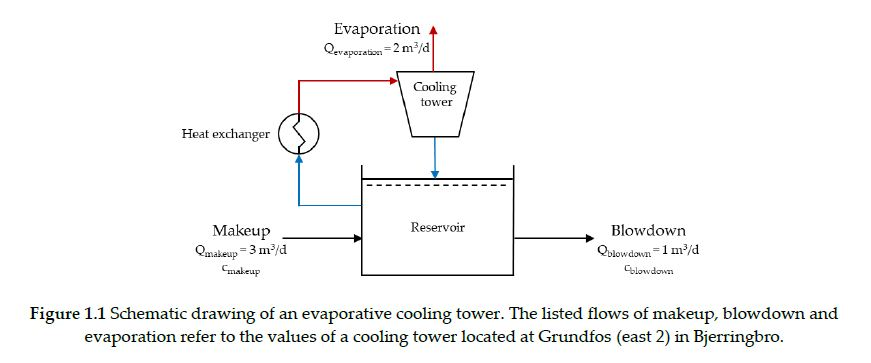
\includegraphics[width=1\textwidth]{Billeder/intro/sebastian_CT_principle.JPG}
    \caption{CT working principle fra spebsatians rap. }
    \label{fig:CT_working_principle}
\end{figure}


%The quality of the cooling water should be considered as dispersed particle or colloids can deposit, scale or block pipes \citep{farahanniRecoveryCoolingTower_2016}. 
The quality of the cooling water should be considered and maintained in order to avoid corrosion, scaling and solid deposition within the tower.  \citep{IntroductionCoolingTower2014}
This is due to the cooling tower design where large quantities of water is lost in the CTs due to evaporation %(high operating temperatures (up to 54 C))
\citep{farahanniRecoveryCoolingTower_2016}, this leads to increase in minerals and contaminants in the cooling water. 
In order to maintain a suitable water quality and water balance a portion of the cooling water must be discharged as waste called blowdown. \citep{IntroductionCoolingTower2014}
The large quantities of water lost due to evaporation and blowdown must be replaced by new cooling water which is called makeup. %this is done in order to maintain the water balance 
\citep{farahanniRecoveryCoolingTower_2016}
Further more as the evaporative CTs are open to the atmosphere various  materials can be introduced into the CT e.g. microorganisms, dirt and dust, this make CTs a possible growth environments for pathogenic microorganism such as legionella.  \citep{IntroductionCoolingTower2014} %(mere om den legionella i kilden).


The water efficiency should also be considered where the relationship between quantity of makeup and blowdown water is typically expressed as cycles of concentration (COC). 
COC describes the total amount of minerals which are concentrated in the cooling water compared to the concentration in the makeup water, or the volume described by equation \ref{eq:COC_eq}. \citep{IntroductionCoolingTower2014}
Higher COC means better water use efficiency, where a COC of 3 is acceptable water efficiency COC of 10 is considered great water efficiency. %a range of 5-7 COC most cost-effective. 
Typically chloride concentration or conductivity is used to calculate the COC. 
\citep{IntroductionCoolingTower2014}


\begin{ceqn}
    \begin{align}
    \label{eq:rejection_formula}
       COC = \frac{ Q_{makeup}}{ Q_{blowdown}}= \frac{ C_{blowdown}}{Q_{makeup}}
    \end{align}
    \label{eq:COC_eq}
\end{ceqn}

\textcolor{red}{Noter til afsnittet: skriv færdig om vandkvalitet, hvad er limit guidlines, hvad er make up vand, få introduceret ioner, hvilke problmer der er med vand når det scaler. Få introduceret problemet med vandkvalitet. noget med at vandkvalitet ændre sig og det ændre COC/operation af CT}


Deposits within a CT can be scaling or fouling, this can interfere with the heat transfer and thus reduce operation efficiency. \citep{IntroductionCoolingTower2014}


Scaling is formed by minerals dissolved in the cooling water, most common scaling minerals are calcium carbonate, calcium phosphate, calcium sulfate and silica. Where most often the minimum salt which control the COC is calcium carbonate, calcium phosphate or silica %in that order. 
\citep{IntroductionCoolingTower2014}
Silica will scale in cool parts of the CT, and calcium salts will scale in warm part of the CT \citep{IntroductionCoolingTower2014}
The COC used for operation is typically determined from the salt which first come out of solution and thus scale on the system.\citep{IntroductionCoolingTower2014} 
Therefore CT manufactures have guidelines for max. concentration of various minerals and contaminants in the CT %kilde
\textcolor{blue}{Noget med quidelines for producenter. }

\begin{table}[h]
\centering
\caption{Guidelines water quality, for Galvanized stell, den er mest følsom.  steel
\url{https://www.evapco.com/sites/evapco.com/files/2017-05/113G.cooling_towers_operation_and_maintenance.pdf}
\url{https://www.baltimoreaircoil.com/download_api_endpoint/1218/partsguide_201710.pdf} } 
\begin{tabular}{c|cc}
Property             & \multicolumn{2}{c}{Manufacturer}\\ \hline
 & Evapco &  Baltimore Aircoil       \\ \hline
pH                      & 7-8.8         & 6.5-9.0\\
total suspended solid  [ppm]& <25       & 25        \\
TDS                     & -             & 15000     \\
Conductivity mu mS/cm   & <2400         & 2400      \\
Alkalinity CaCO2 [ppm]  & 75-400        & 500       \\
 Hardness CaCO2 [ppm]   & 50-500        & 500-600   \\
Chloride [ppm]          & <300          & 250       \\
Silica                  & <150          & 150       \\   
Sulfates                & -             & 250       \\
Bacteria                & <10 000       &           \\
\end{tabular}
\label{Tab:CT_water_threshhold}
\end{table}



\begin{table}[h]
\centering
\caption{\textbf{NB! Fortyndet til 1000 uS cm}Ionic Composition of CT water \textcolor{magenta}{kilde: Grundfos Internal Analyses}}
\begin{tabular}{c|cc}
Ion               & Concentration {[}mg/L{]} & Concentration {[}mM{]} \\ \hline
\ce{HCO3-}        & 444.4                    & 7.29               \\
\ce{Cl-}          & 87.8                     & 2.48               \\
\ce{SO4^2-}       & 61.4                     & 0.64               \\
\ce{Na+}          & 248.6                    & 10.81              \\
\ce{Ca^2+}        & 14.16                    & 0.35               \\
dissolved silica  & 41.13                    & 0.68              
\end{tabular}
\label{Tab:CT_water_composition}
\end{table}

The problematic ions which constitute most of the make up water is \ce{Ca^{2+}}, \ce{Cl-}, \ce{SO_4^{2-}} and \ce{SiO2}.
Where \ce{SO_4^{2-}} (sulphate) is a good indicator for general conductivity in the thank and thus general rejection, see \cref{fig:sulphate_chlroide_concentration_batch} for concentration profile. 
Previous work (by Sebastian) have indicated problems with low rejection and also negative rejection for both \ce{Cl-} and \ce{SiO2}.


Previously blowdown water was simply discharged to surface water without treatment leading to environmental contamination \citep{farahanniRecoveryCoolingTower_2016}
Water scarcity and increasing water prices have been motivation for research in reuse of blowdown as makeup. \citep{farahanniRecoveryCoolingTower_2016}. 
Apart from decreasing the water usage there are other important factors to consider when treating the water for CT. Firstly to  maintain operation efficiency, protect the CT equipment from,  corrosion, deposition and microbial growth. Furthermore the environmental impact should be considered and chemical cost. \citep{IntroductionCoolingTower2014}


% Water led from a reservoir is sprayed into the tower where some of it evaporates and the rest is returned to the reservoir.


% In order to replace the water that evaporates so called 'makeup water'(of a quality similar to tap water) is led into the reservoir at a rate that matches the loss due to evaporation.
% Due to this there is a buildup of species in the water as only pure water escapes by vaporization.
% To ensure proper water quality (ion concentrations) there is a removal stream from the reservoir the so called 'blowdown water'. 


% Cooling tower systems is the process which consume the largest water quantity with regard to petrochemicals, refinereies and power plants. \citep{farahanniRecoveryCoolingTower_2016}



% work to remove heat from a process by evaporation of water.







Membrane technology is burgeoning as a viable option for treatment of the waste water from cooling towers, thus decrease water usage. The membrane processes could be reverse osmosis, electrodialysis, brine concentratior crystallizer and spray dryers. \citep{kaliappan_RecoveryReuseWater_2005} 
Membrane filtration pose as effective process to remove soluble and insoluble organic and inorganic contaminants in waste waters where NF and RO is suggested for use in treating cooling tower blow down water. \citep{farahanniRecoveryCoolingTower_2016}


\rod{Kort ned på generel membran teori, få introduceret case study/kilder omkring membran filtrering af CT vand, fokus på NF mod RO, argumenter for at vi vælger NF, Husk at gem til gammel skrald}

\section{Membrane Filtration Processes}
Pressure driven membrane filtration are processes typically used for treatment of water.
These processes utilise an applied pressure as a driving force in the separation of a fluid stream over a semipermeable membrane. 
The feed stream is divided into a permeate stream which ideally is pure water and a retentate stream containing an increased amount of retained contaminants/solutes. 
Multiple types of pressure driven membrane filtration exist which can be categorised based on their pore size. 
Microfiltration (MF) has the largest pore size, ultrafiltration (UF) has a smaller pore size, and these use micro sieving for contaminant removal.
Nanofiltration (NF) and Reverse Osmosis (RO) membranes are semipermeable and have much smaller pores if they have distinct pores at all, and use diffusion controlled transport mechanisms to remove contaminants.
This is what allows them to filter out ions from the water.

The different membrane types typically have differing characteristics and fields of application, however for some the types there are less clear boundaries e.g. NF filtration can be seen as a mixture between UF and RO filtration processes.\citep{keo}
An overview of the different processes can be seen in \Cref{fig:membrane_values}  
NF membranes allow the retention of ions like in RO filtration but has distinct pores like UF membranes. %mangler kilde
However, monovalent ions are not completely retained and may pass the semi-permeable membrane but di- and tri- valent ions are better retained. 
As NF membranes have a larger poresize than RO, less applied pressure is required to drive water through the membrane, and they are generally less prone to fouling. \citep{keo}
\rod{mangler kilde: As NF require lower operation pressure it is cheaper something something.}

\begin{figure}[H] % (alternativt [htbp])
	\centering
	\def \f {2.235}
\def \d {0.3}
    \pgfplotsset{compat=1.16,width = 15cm,height=9cm}
% \begin{tikzpicture}
%     \begin{semilogxaxis}[log ticks with fixed point]
%         [
%             scale only axis,
%           % ymin=0.4, ymax=2.1,
%             xmin=1e-4, xmax=0.1,
%         ]
%         \addplot {2};
%     \end{semilogxaxis}        
% \end{tikzpicture}


\begin{tikzpicture}[scale=0.8]
\coordinate (A) at (2.235,1);
\coordinate (B) at (2.98,1);
  \begin{semilogxaxis}[
  axis background/.style={fill=gray!10},
    xmin=0.0001, xmax=100,
    ymin=0, ymax=10,
    log basis x=10,
    log ticks with fixed point,
    ytick=\empty,
    xlabel=Particle size ($\mu m$),
    grid=major,
    ]
  % \addplot[mark=*] coordinates {
  % (0.1,6)};
    \node[label={0:{\scriptsize{Coronavirus}}},diamond,fill,inner sep=1.5pt] at (axis cs:0.08,6) {};
    
     \node[label={100:{\scriptsize{             Bacteriophage MS2}}},diamond,fill,inner sep=1.5pt] at (axis cs:0.027,6.4) {};
    
    \node[label={315:{\scriptsize{E. coli}}},diamond,fill,inner sep=1.5pt] at (axis cs:1.2,6) {};
     
     \node[label={0:{\scriptsize{Enterococci}}},diamond,fill,inner sep=1.5pt] at (axis cs:1.6,6.4) {};
    
     \node[label={45:{\scriptsize{Rotavirus}}},diamond,fill,inner sep=1.5pt] at (axis cs:0.072,6.4) {};
     
      \node[label={60:{\scriptsize{Yersinia}}},diamond,fill,inner sep=1.5pt] at (axis cs:0.65,6.4) {};
      
      \node[label={90:{\scriptsize{$Cl^{-}$}}},diamond,fill,inner sep=1.5pt] at (axis cs:0.000181,6.4) {};
      
      \node[label={315:{\scriptsize{$SO_4^{2-}$}}},diamond,fill,inner sep=1.5pt] at (axis cs:0.000242,6.4) {};
  \end{semilogxaxis}
%long rectangles
  \filldraw[gray!30] (0.016,\d)rectangle(13.41,3*\d);
  \filldraw[magenta!100!white!50] (0.016,4*\d)rectangle(5.2*\f,6*\d);
  \filldraw[magenta!100!white!50] (3.9*\f,0.1+6*\d)rectangle(6*\f,0.1+8*\d);
%filtration
  \filldraw[violet!70] (0.016,\d) rectangle (\f,3*\d);
  \filldraw[violet!70] (0.016+\f,\d) rectangle (2.35*\f,3*\d);
%  \filldraw[green!50!black] (0.016+5*\f,\d) rectangle (6*\f,3*\d);
  \filldraw[violet!70] (0.016+2.8*\f,\d) rectangle (5*\f,3*\d);
%Filtrate  
  \filldraw[cyan!70!black] (0.016,9*\d) rectangle (0.6*\f,11*\d);
  \filldraw[cyan!70!black] (0.95*\f,9*\d) rectangle (2.3*\f,11*\d);
  \filldraw[cyan!70!black] (2.4*\f,9*\d) rectangle (3.4*\f,11*\d);
  \filldraw[cyan!70!black] (3.5*\f,9*\d) rectangle (4.95*\f,11*\d);
  \filldraw[cyan!70!black] (5.3*\f,9*\d) rectangle (6*\f,11*\d);  
%nodes 
    \draw (0.5*\f,2*\d) node {RO NF};
    \draw (1.65*\f,2*\d) node {UF};
    \draw (3.9*\f,2*\d) node {MF};
%    \draw (5.5*\f,2*\d) node {P/F?};
    \draw (2.75*\f,5*\d) node {Membranes};
    \draw (5*\f,0.1+7*\d) node {Fibrous Media};
    \draw (0.25*\f,+10*\d) node {Ions};
    \draw (1.6*\f,10*\d) node {Proteins};
    \draw (2.9*\f,10*\d) node {Viruses};
    \draw (4.2*\f,10*\d) node {Bacteria};
    \draw (5.65*\f,10*\d) node {Pollens};
    
\draw (6.705,8) node {Filtration and selected species};
  %\draw (2.24/2,
  \end{tikzpicture}
	\caption{ membrane cut off}
	\label{fig:membrane_values}
\end{figure}

\section{NF Process in CTs}

\rod{Calcium, Sodium, sulphate, Chloride Silica, fokus på chloride + silica, 
målt på rejection af membrane performance, samt hvor meget vand kan vi bespare, det skal være øknomoisk forsvareligt. ikke for disco agtigt.}

%Basically problemet / scope der skal komme ned til PF
%opkoncentrering -> ionbalance/transport af nogle ioner.
%hvor skal spildet hen?
%hvordan kan det betale sig?
The implementation of a filtration process like NF in the CT adds some benefit to the overall operation which has to outweigh the cost of the addition/change in workflow.%hvordan finder man en kilde til sådan noget
Filtration of a reservoir stream should naturally reduce the volume of water that is discarded from the system, which likely would be a benefit as a reduction in water usage would save money.
However the reduction in volume results in wastewater of a much greater concentration which may be more difficult or expensive to discard depending on cost and regulations declared by local municipalities.

The filtration process may also be more complicated than initially apparent and require specific process regulation for optimal performance.
One major reason for this is the nature of how ions are transported though NF membranes and their behaviour at high concentrations near the membrane surface.
Typical composition of reservoir water from CTs is presented in \cref{Tab:CT_water_composition}.
As filtration progresses ions will accumulate at the membrane wall and if the filtration is carried out as a batch process the concentration of ions will also increase in the feed container.
This accumulation will affect membrane performance and may, depending on feed composition, reduce the quality of produced permeate.%kilde mangler

Previous work \rod{Sebastians rapport AAU} has shown that membrane rejection for specific ions changes quite dramatically as the concentration increases exemplified by \ce{Cl-} which was shown to have negative rejection at high \ce{SO_4^2-} concentrations.
One way to combat this is by running the filtration in multiple batches whereby \ce{SO_4^2-} can be removed from the system before \ce{Cl^-} is filtered.
\textcolor{magenta}{Si scaling problems}




This project work will focus on how certain ions, specifically \ce{Cl-} and \ce{SiO2} are rejected by a NF membrane and how their rejection is impacted by their chemical environment.
This will be done by investigating how they interact with the membrane and how their transport through it is facilitated during a filtration process.


% \textbf{Altman}
% Altman et al.\citep{altmanMembraneTreatmentSidestream2012} used NF for side-stream treatment of a cooling tower. 
% A pilot study run for 3 months on a CT.
% 1200 uS/cm
% scale inhibitor and biocide norm added.
% system had 2 media prefilters to remove pariculates and chlorine + organoics.
% added anti-scalanat.
% membranes were tfc softening membranes with reported >90\% chloride rejection.
% pressure around 8 bar
% saw clear results of irreversible scaling/fouling with flow rates approaching 0 after 90 days.
% scale was determined to mainly be silicon due to the use of anti-scalants with calcium-salts assumed to be more prone to scaling without these additions
% CoC was calculated to increase from 3 to as much as 4.9 with an average being 3.4 and blowdown water could be reduced by as much as 49\% and an average estimate of makeup water saved was 6\% with 16\% being the highest saving possible.
% Recovery was the most important factor.
% high pressure inhibiting due to power consumption/ cost
% membranes with lower rejection rates(70-90\%) but higher recoveries would stand to gain more savings.
% membrane performacne was an rejection of 89-99\% removal of dissolved constituents.

MEMBRANE THEORY. 
Typically pressure driven membranes, which include microfiltration (MF),
ultrafiltration (UF), nanofiltration (NF), and reverse osmosis (RO) are used. 
These membrane processes are listed in order from lower to higher pressure requirements and removal efficiencies, with RO requiring the greatest amount of pressure/energy but being able to remove monovalent ions.\citep{keo} 

noget case study: 
%RO and NF membranes are considered non-porous in that they do not have a well defined pore structure and can exclude low molarmass species. 


% Pressure driven membrane filtration are processes typically used for treatment of water.
% These processes utilise an applied pressure as a driving force in the separation of a fluid stream over a semipermeable membrane. 
% The feed stream is divided into a permeate stream which ideally is pure water and a retentate stream containing an increased amount of retained contaminants/solutes. 
% Multiple types of pressure driven membrane filtration exist which can be categorised based on their pore size. 
% Microfiltration (MF) has the largest pore size, ultrafiltration (UF) has a smaller pore size, and these use micro sieving for contaminant removal.
% Nanofiltration (NF) and Reverse Osmosis (RO) membranes are semipermeable and have much smaller pores if they have distinct pores at all, and use diffusion controlled transport mechanisms to remove contaminants.


%An overview of the different processes can be seen in \Cref{fig:membrane_values}  
%NF membranes allow the retention of ions like in RO filtration but has distinct pores like UF membranes. %mangler kilde
%However, monovalent ions are not completely retained and may pass the semi-permeable membrane but di- and tri- valent ions are better retained. 
%As NF membranes have a larger poresize than RO, less applied pressure is required to drive water through the membrane, and they are generally less prone to fouling. \citep{keo}
%\rod{mangler kilde: As NF require lower operation pressure it is cheaper something something.}



gamle case study afsnit: 

This viability was tested in \citep{altmanMembraneTreatmentSidestream2012} where a pilot-scale experiment concerning NF treatment of BD was conducted.
The experiment ran for three months and found that the maximum water savings for the CT were 16\% and 49\% for the make-up and blowdown respectively.
The actual water saving was much lower due to high degree of scaling on the membranes, primarily due to silica and calcium salts.
The membrane performance was 89-99\% removal of dissolved constituents.
This is in good agreement with \citep{kaliappan_RecoveryReuseWater_2005} which also used NF to treat CT BD water.
They found salt rejections of 87 - 89 \%.
It was noted that such high rejections are unnecessary and that membranes with lower rejection rates(70-90\%) but higher recoveries would better suited for use with CTs.
Both studies also noted fouling as a major problem.


There has also been multiple studies on implementing RO membranes in the same manner for treatment of CT blowdown.
Using discarded RO membranes for treatment of blowdown stream have been investigated by \citep{frickEvaluationPretreatmentsBlowdown2014}.
They were deemed appropriate for CT BD filtration as characterization of the discarded RO membranes determined their performance to be similar to NF membranes.
\citep{farahanniRecoveryCoolingTower_2016}investigated and compared RO and NF filtration for the purpose of recovering water from CT BD streams along with evaluating different pre-treatments.
The RO membrane shoved better rejection of TDS and COD removal, however it was commented that the increased operational costs of RO make them difficult to recommend over NF for use as side-stream treatment in CTs.
Both RO and NF systems required pre-filtration to avoid fouling and it was generally apparent that the RO membranes required a more thorough pre-filtration to make them viable.
Coagulation/flocculation was shown to be the most efficient method increasing permeate flux by 25\% and 33\% for NF and RO respectively.
Using MF or UF membranes as pre-treatment options for BD treatment was investigated in \citep{zhangPilotTestingOutsidein2007,zhangPilotTestUF2008}  
Other types of technologies often implemented in desalination have also been investigated in regards to treatment of CT wastewater.
\textbf{Liao et al.} and \textbf{Silvia Lucila et al.} used electrocoagulation to remove ions. 
Mainly silica and calcium which were deemed the most troublesome ions for CT operation from cooling tower blowdown water.

mere case study 
 \prettyinpink{nedenstående argument føler jeg at vi har manglet et eller andet sted}
% "Predictive calculations [9] indicated that ultrapurewater (>90\% chemical
% rejection)was not necessary for optimal water savings in this application."


% \textbf{Random patent-gut}
% Jones Randall J. has a patent pertaining to a purification system for cooling towers using NF and ionization to reduce discharge volume by 80\% and remove the need for anti-scalant chemicals% also uses sand filter and "a disinfection unit". is from 1991 so NF membranes may have been hot garbage at that point.


%In most industrial processes temperature control is needed \citep{ReviewStudyCoolingtower_2019}. 
%There exists different types of cooling water systems, a common type is open recirculating cooling towers, where the water is recirculated multiple times and the system is open to the atmosphere.
%This type of CT is a suitable method for dissipation of excess heat in majority of cases \citep{PlantEngineerBookReference2001}. 
% https://www.suezwatertechnologies.com/handbook/chapter-31-open-recirculating-cooling-systems
%The open recirculating CT cools water by evaporation \citep{PlantEngineerBookReference2001}, 
%where some water evaporates and due to the latent heat of vaporization the temperature of the remaining water decreases. %kilde steffen?. evt. atkins. 
%about 70-80\% of the cooling is due to evaporative cooling, and the remaining 20-30\% is due to conductive heat transfer. \citep{IntroductionCoolingTower2014} 
%The cooled water is recirculated to heat exchangers where heat is transferred to the cooling water from the given industrial process. 
%The heated water is reintroduced into the cooling tower where the evaporation cycle is repeated, this process is illustrated in \cref{fig:CT_working_principle}. \citep{IntroductionCoolingTower2014} 
%The quality of the cooling water should be considered as dispersed particle or colloids can deposit, scale or block pipes \citep{farahanniRecoveryCoolingTower_2016}. 
%Due to the large quantities of evaporated water this leads to increase in concentration of salts, minerals and other contaminants in the cooling water \citep{koemanMembraneDistillationIndustrial2016}. 


%The quality of the cooling water should be considered and maintained in order to avoid corrosion, scaling and solid deposition within the tower.  \citep{IntroductionCoolingTower2014}
%In order to maintain a suitable water quality and water balance a portion of the cooling water must be discharged as waste called blowdown. \citep{IntroductionCoolingTower2014}
%The large quantities of water lost due to evaporation and blowdown must be replaced by new cooling water which is called makeup. %this is done in order to maintain the water balance 
%\citep{farahanniRecoveryCoolingTower_2016} \citep{koemanMembraneDistillationIndustrial2016}. 
%As the evaporative CTs are open to the atmosphere various  materials can be introduced into the CT e.g. microorganisms, dirt and dust, this make CTs a possible growth environments for pathogenic microorganism such as legionella.  \citep{IntroductionCoolingTower2014} %(mere om den legionella i kilden).


% \textbf{Altman}
% Altman et al.\citep{altmanMembraneTreatmentSidestream2012} used NF for side-stream treatment of a cooling tower. 
% A pilot study run for 3 months on a CT.
% 1200 uS/cm
% scale inhibitor and biocide norm added.
% system had 2 media prefilters to remove pariculates and chlorine + organoics.
% added anti-scalanat.
% membranes were tfc softening membranes with reported >90\% chloride rejection.
% pressure around 8 bar
% saw clear results of irreversible scaling/fouling with flow rates approaching 0 after 90 days.
% scale was determined to mainly be silicon due to the use of anti-scalants with calcium-salts assumed to be more prone to scaling without these additions
% CoC was calculated to increase from 3 to as much as 4.9 with an average being 3.4 and blowdown water could be reduced by as much as 49\% and an average estimate of makeup water saved was 6\% with 16\% being the highest saving possible.
% Recovery was the most important factor.
% high pressure inhibiting due to power consumption/ cost
% membranes with lower rejection rates(70-90\%) but higher recoveries would stand to gain more savings.
% membrane performacne was an rejection of 89-99\% removal of dissolved constituents.




% \textbf{Kaliappan et al.}\citep{kaliappan_RecoveryReuseWater_2005}
% used ultra low pressure RO (AKA. NF) for treatment of BD water from a fertilizerr unit'
% 5um and 1 um prefilter follwed by carbon filter.
% even with all pretreatment fouling was still observed.
% pressure was varied from 2.75 to 4.13 bar
% \begin{align}
%     CoC=100/(100-Recovery)
% \end{align}
% feed conductivity was 3350, TDS 2500, 
% Salt rejection increased with feed pressure.
% Salt rejection and permeate flux increased with recovery %how was recovery changed at constant pressure? -det er single pass?   
% salt rejection was 89\% at 4.13 bar and recovery was 56\%.




% \begin{figure}[H] % (alternativt [htbp])
% 	\centering
% 	\def \f {2.235}
\def \d {0.3}
    \pgfplotsset{compat=1.16,width = 15cm,height=9cm}
% \begin{tikzpicture}
%     \begin{semilogxaxis}[log ticks with fixed point]
%         [
%             scale only axis,
%           % ymin=0.4, ymax=2.1,
%             xmin=1e-4, xmax=0.1,
%         ]
%         \addplot {2};
%     \end{semilogxaxis}        
% \end{tikzpicture}


\begin{tikzpicture}[scale=0.8]
\coordinate (A) at (2.235,1);
\coordinate (B) at (2.98,1);
  \begin{semilogxaxis}[
  axis background/.style={fill=gray!10},
    xmin=0.0001, xmax=100,
    ymin=0, ymax=10,
    log basis x=10,
    log ticks with fixed point,
    ytick=\empty,
    xlabel=Particle size ($\mu m$),
    grid=major,
    ]
  % \addplot[mark=*] coordinates {
  % (0.1,6)};
    \node[label={0:{\scriptsize{Coronavirus}}},diamond,fill,inner sep=1.5pt] at (axis cs:0.08,6) {};
    
     \node[label={100:{\scriptsize{             Bacteriophage MS2}}},diamond,fill,inner sep=1.5pt] at (axis cs:0.027,6.4) {};
    
    \node[label={315:{\scriptsize{E. coli}}},diamond,fill,inner sep=1.5pt] at (axis cs:1.2,6) {};
     
     \node[label={0:{\scriptsize{Enterococci}}},diamond,fill,inner sep=1.5pt] at (axis cs:1.6,6.4) {};
    
     \node[label={45:{\scriptsize{Rotavirus}}},diamond,fill,inner sep=1.5pt] at (axis cs:0.072,6.4) {};
     
      \node[label={60:{\scriptsize{Yersinia}}},diamond,fill,inner sep=1.5pt] at (axis cs:0.65,6.4) {};
      
      \node[label={90:{\scriptsize{$Cl^{-}$}}},diamond,fill,inner sep=1.5pt] at (axis cs:0.000181,6.4) {};
      
      \node[label={315:{\scriptsize{$SO_4^{2-}$}}},diamond,fill,inner sep=1.5pt] at (axis cs:0.000242,6.4) {};
  \end{semilogxaxis}
%long rectangles
  \filldraw[gray!30] (0.016,\d)rectangle(13.41,3*\d);
  \filldraw[magenta!100!white!50] (0.016,4*\d)rectangle(5.2*\f,6*\d);
  \filldraw[magenta!100!white!50] (3.9*\f,0.1+6*\d)rectangle(6*\f,0.1+8*\d);
%filtration
  \filldraw[violet!70] (0.016,\d) rectangle (\f,3*\d);
  \filldraw[violet!70] (0.016+\f,\d) rectangle (2.35*\f,3*\d);
%  \filldraw[green!50!black] (0.016+5*\f,\d) rectangle (6*\f,3*\d);
  \filldraw[violet!70] (0.016+2.8*\f,\d) rectangle (5*\f,3*\d);
%Filtrate  
  \filldraw[cyan!70!black] (0.016,9*\d) rectangle (0.6*\f,11*\d);
  \filldraw[cyan!70!black] (0.95*\f,9*\d) rectangle (2.3*\f,11*\d);
  \filldraw[cyan!70!black] (2.4*\f,9*\d) rectangle (3.4*\f,11*\d);
  \filldraw[cyan!70!black] (3.5*\f,9*\d) rectangle (4.95*\f,11*\d);
  \filldraw[cyan!70!black] (5.3*\f,9*\d) rectangle (6*\f,11*\d);  
%nodes 
    \draw (0.5*\f,2*\d) node {RO NF};
    \draw (1.65*\f,2*\d) node {UF};
    \draw (3.9*\f,2*\d) node {MF};
%    \draw (5.5*\f,2*\d) node {P/F?};
    \draw (2.75*\f,5*\d) node {Membranes};
    \draw (5*\f,0.1+7*\d) node {Fibrous Media};
    \draw (0.25*\f,+10*\d) node {Ions};
    \draw (1.6*\f,10*\d) node {Proteins};
    \draw (2.9*\f,10*\d) node {Viruses};
    \draw (4.2*\f,10*\d) node {Bacteria};
    \draw (5.65*\f,10*\d) node {Pollens};
    
\draw (6.705,8) node {Filtration and selected species};
  %\draw (2.24/2,
  \end{tikzpicture}
% 	\caption{ membrane cut off}
% 	\label{fig:membrane_values}
% \end{figure}